% !TeX root = ../main.tex
% !TEX root = ../main.tex
% -*- root: ../main.tex -*-
% -*- program: pdflatex -*-
\chapter{前言}

\section{粒子物理}
物质组成的最小单位是什么?这是人们探索自然界的普遍规律时关心的问题。中国夏朝有“五行学说”,认为物质是由金、木、水、火、土组成;而古希腊有物质是由水、火、土、空气四种元素组成的“四元素学说”。19世纪,自然科学创立,物理、化学等领域相继诞生。19世纪初,道尔顿(John Dalton,1766-1844)提出原子论,认为物质是由一种单一的粒子组成的~\cite{cite1:lv}~。 19~世纪初,道尔顿(~John~Dalton,~1766~-~1844~)~提出原子论,认为物质是由一种单一的粒子组成的。19世纪末,英国物理学家汤姆逊通过真空管阴极射线实验发现了电子。20~世纪物理学物理学得到了极大地发展,量子力学和相对论相继建立并蓬勃发展,各种粒子相继被发现。例如~1897~年汤普逊发现电子;1901~年普朗克提出光量子假说,之后的~1905~年爱因斯坦利用此假说成功解释了光电效应;1911~年卢瑟福提出原子的核式结构,并于~1919~年发现了p;1932~年查德威克发现了中子;1932~年发现了第一个反粒子正电子;1937~年发现~$\mu$~子;1947~年发现~$\pi$~介子;1950~年发现~$K$~介子,$\Lambda$,$\Sigma$;1955~年发现反质子;1956~年发现反中子;1974~年发现~$J/\Psi$~介子,证实了粲(c)夸克的存在;1975~年发现~$\tau$~轻子;1983~年发现玻色子:$W^{\pm}$~和~$Z^{0}$;1995~年发现顶夸克(top);2012~年发现希格斯(~Higgs~)粒子~\cite{ATLAS:2012}\cite{CMS:2012}。基本粒子的发现和研究,加快了粒子物理学的发展进程。
\begin{table}[!htb]
    \centering
    \caption{\label{tbl:interaction} 四种基本相互作用性质的比较}
    \footnotesize
    \begin{tabular}{llllll}
        \hline
        相互作用& 源&     相互作用常数&                   媒介子&                            典型作用时间&   力程 \\
        \hline
        强作用&   色荷&   $\cong$ 1~10&                 胶子(g)&                           $10^{-23}$s&    1fm \\
        电磁作用& 电荷&   $\cong$ 1/137&                 光子($\gamma$)&                    $10^{-16}$s&    $\infty$\\
        弱作用&   弱超荷& $\cong$ $10^{-5}$&             中间玻色子($W^{\pm}$,$Z^{0}$)&      $10^{-10}$s&   1/400fm \\
        引力&     质量&   $\cong$ 5$\times 10^{-40}$&    $\text{---}$&                      ---&           $\infty$\\
        \hline
    \end{tabular}
\end{table}

粒子物理学又称高能物理,是研究基本粒子的性质、运动、相互作用、相互转化的规律的学科,是物理学的基础学科,也是物理学研究的最前沿\cite{cite2:zhang}。自然界存在四种基本的相互作用:强相互作用、弱相互作用、引力相互作用、电磁相互作用,粒子物理主要研究对象是除引力以外的其他三种相互作用。四种基本相互作用的性质如表~\ref{tbl:interaction}~所示。标准模型(Standard~Model,~SM)~是目前描述基本相互作用以及基本粒子最成功的理论\cite{cite3}。标准模型认为物质的最基本结构是夸克、轻子以及相互作用传播子。夸克按性质和质量可以分成三代,分别为(u,d)、(c,s)、(t,b),具有分数电荷;轻子也分为三代,分别是($e^{-}$,  $\nu^{e}$)、(~$\mu^{-}$, $\nu^{\mu}$)、($\tau^{-}$,$\nu^{\tau}$)。每一种夸克和轻子都有相应的反粒子;光子是电磁相互作用的传播子,$W^{\pm}$~及$Z^{0}$粒子是弱相互作用的传播子,胶子是强相互作用的传播子; Higgs 粒子是对称性自发破缺的源头,使得规范玻色子和费米子具有了质量。图~\ref{fig:standard_model_particle}~是基本粒子的示意图。
\begin{figure}[!h]
  \centering
  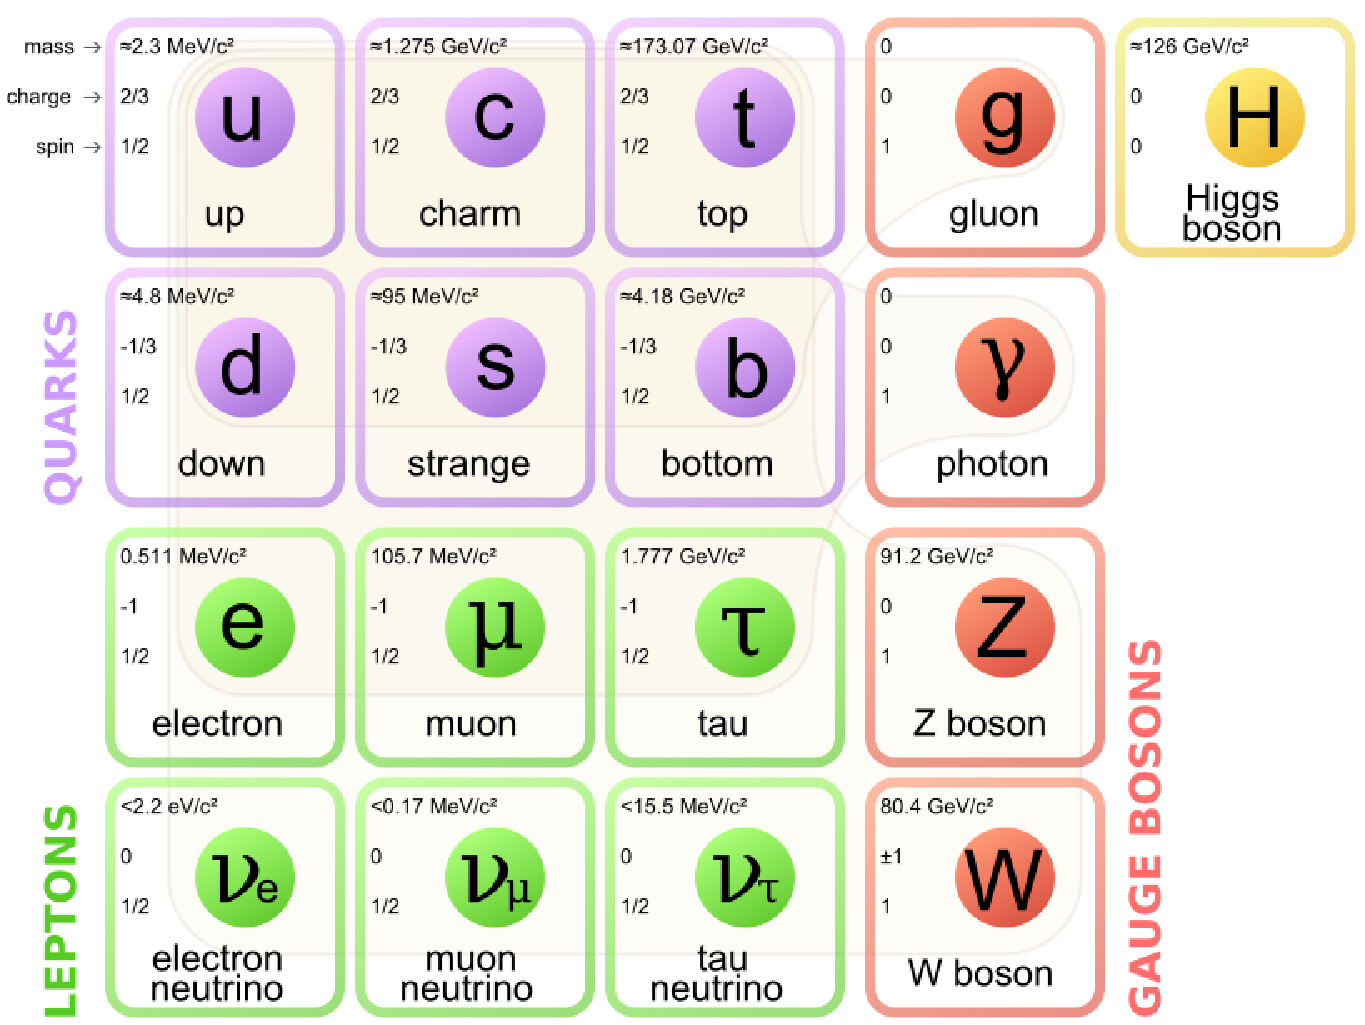
\includegraphics[width=10cm]{chap0/Standard_Model_of_Elementary_Particles.pdf}
  \caption{标准模型中的基本粒子}
  \label{fig:standard_model_particle}
\end{figure}

粒子物理是一门实验学科。研究微观粒子需要很高的能量,因此需要高能加速器和探测器。对撞机在高能物理中有着十分重要的地位。$J/\psi$~粒子、$\tau$~轻子和~$\Upsilon$~粒子都可以在对撞实验中被发现,高能量的~$Z^{0}$~粒子、$W^{\pm}$~粒子、t夸克和~higgs~粒子也都是在对撞实验中被发现的。表~\ref{tbl:collider-accelerator}~列出了世界上主要的加速器及其研究重点。
\begin{table}[h]
    \centering
    \caption{\label{tbl:collider-accelerator} 主要高能物理对撞机及其研究重点}
    \footnotesize
    \begin{tabular}{lllll}
        \hline
        名称& 国家& 粒子源& 能量(~Gev~)& 研究重点\\
        \hline
        BEPC(BEPCII)& 中国& $e^{+}$/$e^{-}$& 2~5& 粲夸克、$\tau$粲能区物理 \\
        CESR& 美国& $e^{+}$/$e^{-}$& 10& b夸克 \\
        CESR-c& 美国& $e^{+}$/$e^{-}$& 3-11& 粲偶素、D物理 \\
        HERA& 德国&  $e^{-}$/$\overline{p}$&30/820& 质子结构\\
        TEVATRON& 美国& p/p&1800& t夸克\\
        PEPII& 美国& $e^{+}$/$e^{-}$& 3.1/9& b介子、CP破坏\\
        KEKB& 日本&   $e^{+}$/$e^{-}$& 3.5/8& b介子、CP破坏\\
        RIHC& 美国& $A_{u}$/$A_{u}$& 200& 重离子对撞\\
        LHC& 瑞士(CERN)& p/p(Pb/Pb)& 14000(2700)& Higgs、b介子、CP破坏、重离子\\
        \hline
    \end{tabular}
\end{table}



\section{环形正负电子对撞机~(CEPC)~}
\subsection{CEPC提出背景}
希格斯粒子\cite{higgs1}\cite{higgs2}是为了解释物质的质量起源而被提出来的。它自旋为零,自身的质量来源还待进一步研究,参与非规范相互作用。希格斯粒子和其自身的相互作用对宇宙早期演化具有重要的影响。希格斯粒子由于十分重要被称为“上帝粒子”,对希格斯粒子的研究能引导粒子物理和其他理论的发展,最终可能引起新物理、新技术的发展。希格斯粒子在二十世纪六十年代被提出,但当时对撞机的能量无法满足产生希格斯粒子的要求,所以不能从实验证实希格斯粒子的存在。直到2012年7月4日,欧洲核子中心(CERN)发布了其两个探测器独立探测到疑似希格斯粒子的消息\cite{cern1}\cite{cern2}\cite{cern3}:CMS探测到一种质量为 125.3 $\pm$0.6GeV/$c^{2}$ 的未知玻色子,如图~\ref{fig:cms_higgs}~所示\cite{cern4};ATLAS 探测到质量为126.5GeV/$c^{2}$ 的未知玻色子\cite{cern5}。这一消息引起了粒子物理界的巨大轰动。之后经 LHC 进一步证实,确认了新发现的波色子就是希格斯粒子。希格斯粒子的发现,标志着标准模型预测的粒子被全部发现。然而高能物理科学家普遍相信,标准模型并不是粒子物理的终极理论,我们仍需探索标准模型之外的新物理。
\begin{figure}[!h]
  \centering
  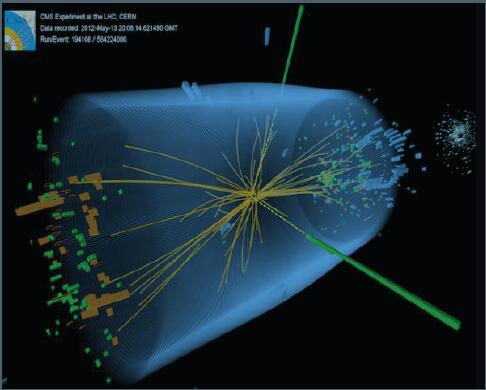
\includegraphics[width=10cm]{chap0/higgs_cms.jpg}
  \caption{CMS捕获的Higgs粒子}
  \label{fig:cms_higgs}
\end{figure}

为了探索超出标准模型之外的新物理,需要有更高能量的探测器。目前对Higgs粒子进行研究的是欧洲大型强子对撞机( Large Hardron Collider, LHC ), LHC由于是质子对撞机,所以对撞产生粒子的能量很高,使其具有很强的发现新物理的能力。 但由于强子对撞过程复杂,产生很大的本底,不利于对希格斯粒子的测量,并且由于质子不是基本粒子,无法计算对撞时质心的质量。由于以上种种不利因素,使得LHC对希格斯粒子测量时产生很大的误差。想要更加精确地研究希格斯粒子的性质及其作用原理,必须依赖轻子对撞机,建造希格斯工厂对希格斯粒子进行更加精确深入的研究。 

为了推动高能物理学的进一步发展,中国高能物理学界提出了建造高能环形正负电子对撞机( Circular Electron Positron Collider, CEPC ),之后升级为超级强子对撞机( Super Positron Positron Collider, SPPC )的方案。方案示意图如~\ref{fig:cepc_sppc}~所示。2015年,CEPC的设计报告初步完成。,作为希格斯工厂,~CEPC~对撞的质心系能量240-250~GeV,周长为 50-100公里的环形正负电子对撞机,预计每年每个对撞点亮度可达到250$fb^{-1}$ ,它在5$fb^{-1}$的总积分亮度下。十年内可以产生约一百万个希格斯波色子\cite{zhuxuezheng}。
\begin{figure}[!h]
  \centering
  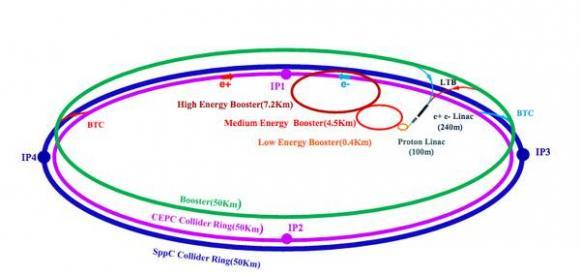
\includegraphics[width=10cm]{chap0/cepc_sppc.jpg}
  \caption{CEPC和SPPC设计图}
  \label{fig:cepc_sppc}
\end{figure}

\subsection{CEPC的主要目标}
CEPC的主要物理目标有:将正负电子加速到250GeV左右对撞,对正负电子对撞后产生的希格斯粒子进行精确测量。在对希格斯粒子研究过程中,深入探究质量起源以及电弱CP破缺机制等基本物理问题,并发现可能超出标准模型之外新物理现象的线索。CEPC运行结束后,在其同一隧道升级为SPPC。SPPC可将对撞粒子的能量加速至50-100TeV,能量超过LHC 能量的~7~倍。SPPC 的主要目标为通过高能量的质子对撞,探索标准模型之外的新物理现象如超对称物理。这将有助于我们队宇宙中的暗物质,暗能量以及宇宙暴胀产生原理形成新的认识,从而能更加深入地了解我们所处的宇宙。\\

\subsection{CEPC模拟软件框架}
目前高能物理对撞机实验设备建造前都需要先对其模拟研究。对于CEPC来说,探测器设计是整个CECP设计中很重要的一环。探测器模拟通过蒙特卡洛( Monte Calo )方法模拟重建粒子产生、运输以及相互作用、响应时间等过程,对探测器的建造进行模拟研究。对探测器的设计和建造来说,探测器模拟具有十分重要的参考价值。探测器模拟可以用于算法研究,参数优化,以及估计探测器的探测效率,其大致流程如图~\ref{fig:sim}~所示。
\begin{figure}[!htb]
  \centering
  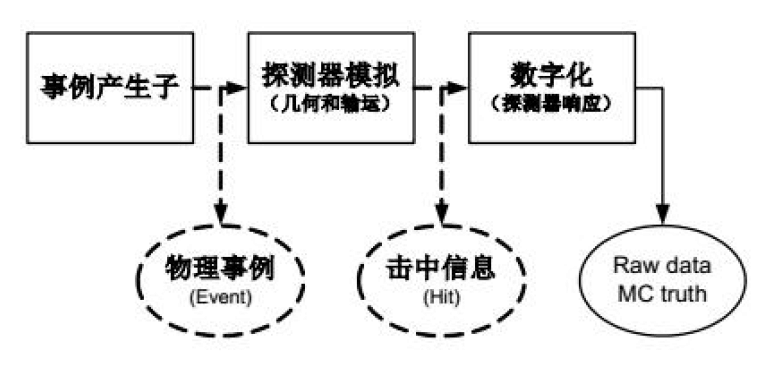
\includegraphics[width=10cm]{chap0/sim.png}
  \caption{探测器模拟重建算法流程图}
  \label{fig:sim}
\end{figure}

在CEPC采用Geant4 作为其探测器模拟的工具。Geant4 是由欧洲核子中心主导开发的一款基于蒙特卡洛的程序包。其可以用来模拟高能粒子的相互作用和在物质中的输运过程。Geant4 的功能涉及到探测器模拟的每一个子过程,如事例产生、几何、物质材料、探测器响应、径迹跟踪、图形显示,用户接口等~\cite{zhuxuezheng}。其功能示意图如图\ref{fig:geant4}~所示。用户可以根据自己的需要选择相应的功能。高能粒子的物理相互作用包含粒子类型以及相互作用类型两个部分。Geant4~提供了各种基本粒子的种类和属性,以及统一的电磁相互作用模型,多种强相互作用模型。除此之外,Geant4 还提供了用于检查Geant4 程序是否正确的可视化接口。
\begin{figure}[!htb]
  \centering
  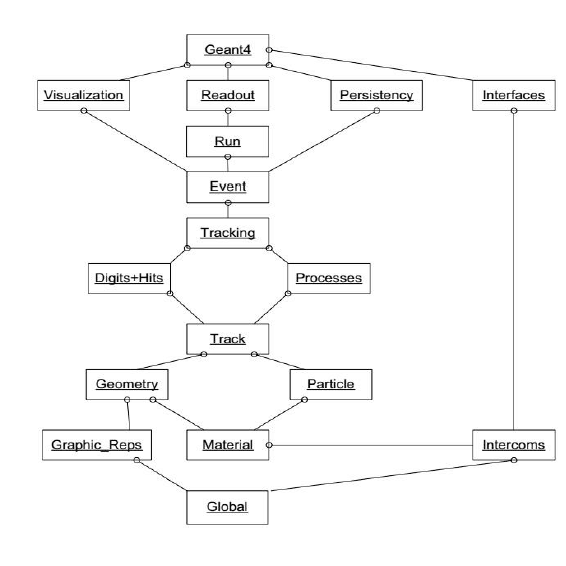
\includegraphics[width=10cm]{chap0/geant4.png}
  \caption{Geant4软件包结构示意图}
  \label{fig:geant4}
\end{figure}

\subsection{CEPC探测器结构}
CEPC探测器包含顶点探测器,时间投影室,硅径迹室,量能器,$\mu$~探测器等若干子探测器,其结构如图\ref{fig:geant4}~所示。其设计方案借鉴了ILC 的设计,并结合自身条件作了一些改变,比如缩小CEPC探测器整体尺寸和探测器的Half~Z 值,改变顶点探测器内半径以及时间投影室外半径等。个子探测器的结构和功能如下:\\
(1). 中心径迹探测器和顶点探测器

顶点探测器和中心径迹探测器的结构如图\ref{fig:vtx}~和图\ref{fig:vtxx}~所示。它们离正负电子对撞点最近,是CEPC整个探测器重要的组成部分,其主要功能有:

(a).确定对撞点的位置。

(b).测量次级粒子衰变的顶点。

(c).测量高能粒子在磁场中偏转的径迹,曲率半径和电荷符号。

(d).测量次级粒子电荷量,并与其它探测器得到的信息相结合,测量粒子的类型和动量。

\begin{figure}[!htb]
  \centering
  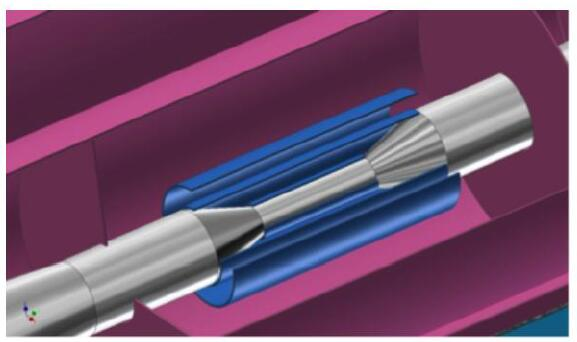
\includegraphics[width=10cm]{chap0/vtx.jpg}
  \caption{顶点探测器}
  \label{fig:vtx}
\end{figure}
\begin{figure}[!htb]
  \centering
  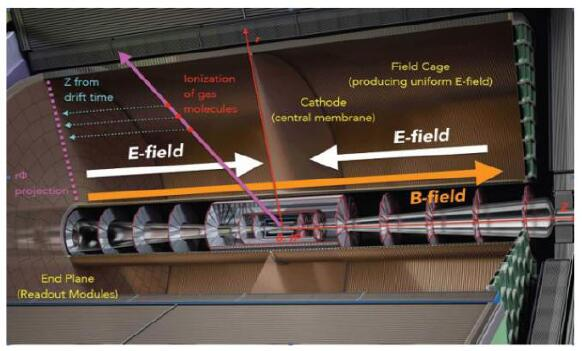
\includegraphics[width=10cm]{chap0/vtxx.jpg}
  \caption{中心径迹探测器}
  \label{fig:vtxx}
\end{figure}
\noindent(2).量能器

量能器的作用为测量高能粒子的位置,能量,飞行方向等物理量。CEPC量能器结构参考ILC~量能器的设计结构(图\ref{fig:energy}~)。量能器能够对粒子能量进行很好地测量,已成为高能物理实验中不可或缺的部分。它具有如下特性:

(a).既能测量带电粒子,又能测量中性粒子。

(b).能够精确地测量入射粒子的方向和位置信息。

(c).能量的测量精度随着入射粒子能量的提高而提高。

(d).对不同的粒子有不同的相应,可用于粒子鉴别。

(e).在能量很高的情况下,可以有较小的尺寸。

(f).时间相应快,可进行高计数工作。

\begin{figure}[!htb]
  \centering
  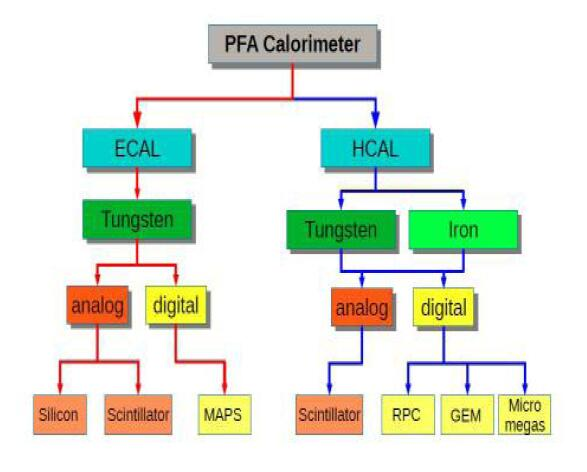
\includegraphics[width=10cm]{chap0/energy.jpg}
  \caption{ILC量能器候选方案}
  \label{fig:energy}
\end{figure}
\noindent(3).$\mu$子探测器

$\mu$子探测器作用为测量$\mu$子的位置,动量等信息,其布局结构如图\ref{fig:muon}~所示。$\mu$子探测器可鉴别出$\mu$子和其它粒子。由于$\mu$子探测器的空间比较大,它可以补偿量能器部分的能量泄漏~\cite{cite1:muon}~。

\begin{figure}[!htb]
  \centering
  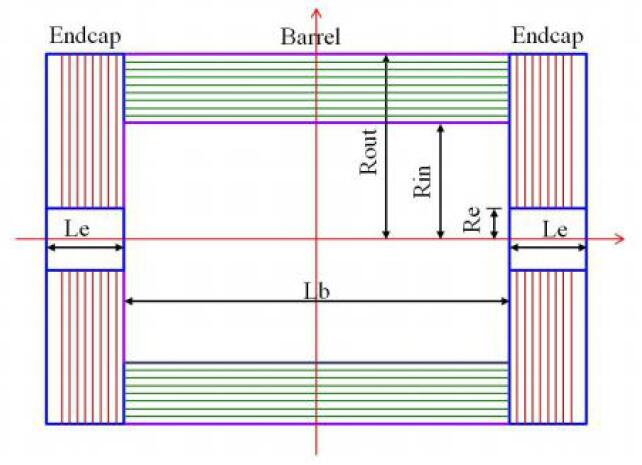
\includegraphics[width=10cm]{chap0/muon.jpg}
  \caption{Muon探测器布局结构}
  \label{fig:muon}
\end{figure}

\section{喷注味道鉴别}
喷注(jet)是指在高能实验中产生的呈喷射状的粒子团~\cite{jet}。喷注味道鉴别( jet flavor tag )是指将喷注中的底(b)夸克, 粲(c)夸克和轻夸克区分开来。虽然标准模型日趋完善,但高能物理学界普遍相信标准模型并不是解释物理现象的终极理论,在更高的能量区间扔有很大的潜力发现新粒子和新的相互作用。而发现新物理依赖于对高能粒子及其相互作用的精确测量。在CEPC 实验中,喷注味道鉴别对测量 Higgs 到 bb,cc 的分支比等物理至关重要,并且可以用来精确检验 Higgs 到费米子对的Yukawa 耦合和其它标准模型性质,比如:Rb(Zbb);同时对于 jet 的研究也会顶点探测器的设计优化提出更多的依据。

\section{机器学习}
机器学习( Machine Learning )是人工智能领域研究的核心内容。它吸收了概率论,信息论,控制论等学科的成果,研究计算机模拟人类的学习行为,以获取新的知识技能并不断完善自身的性能。随着计算机计算能力的提升和算法的发展,机器学习得到越来越广泛的应用,在很多领域(诸如数据挖掘,生物医药,图像识别等)都取得了瞩目的成就。

喷注味道鉴别需要从探测器中读出数据,由于数据具有数据量大,多维度的特点,很难使用传统公式推理的方式。
\section{CEPC喷注味道鉴别}
目前课题所有数据均由蒙特卡洛模拟产生。数据包含3类事例:b夸克,c夸克和其他夸克。每类包含210000事例。每个事例包含68个变量。本课题将所有事例分为训练集(400000个事例),3个验证集(每个验证集包含50000个事例)和测试集(80000事例)。课题使用训练集训练机器学习模型,使用验证集调节各机器学习模型的超参数,然后使用测试集测试各种算法的效果。

\section{机器学习分类器的性能度量}
性能度量( performance measure ) 是衡量模型泛化能力的评价标准。在对比不同的模型时,使用不同的性能度量往往会导致不同的评判结果~\cite{zhouzhihua}。
(1).准确率
精度(accuracy)是指分类器正确分类的样本数占样本总数的比例。
(2).真正例( True Positive, TP ):真实类别为正,预测类别也为正的事例。
假正例( False Postive, FP ):真实类别为负,预测类别为正的事例。
假负例( False Negative, FN ):真实类别为正,预测类别为负的事例。
真负例( True Negative, TN ): 真实类别为负,预测类别也为负的事例。
预测结果的混淆矩阵( confusion matrix )如表~\ref{tbl:confusion_matrix}~所示。
\begin{table}[h]
    \centering
    \caption{\label{tbl:confusion_matrix} 预测结果的混淆矩阵}
    \footnotesize
    \begin{tabular}{|c|c|c|}
        \hline
        %\multirow 纵向合并 \multicolumn横向合并 |c| 两侧添加竖线
        \multirow{2}*{真实情况} & \multicolumn{2}{|c|}{预测结果}\\
        \cline{2-3}
        ~&正例& 反例\\
        \cline{1-3}
        正例& TP(真正例)& FN(假反例)\\
        反例& FP(假正例)& TN(真反例)\\
        \hline
    \end{tabular}
\end{table}
(2).ROC曲线
信号效率()
(3).




